% Copyright (c)  2005-2010 EDF-EADS-PHIMECA.
% Permission is granted to copy, distribute and/or modify this document
% under the terms of the GNU Free Documentation License, Version 1.2
% or any later version published by the Free Software Foundation;
% with no Invariant Sections, no Front-Cover Texts, and no Back-Cover
% Texts.  A copy of the license is included in the section entitled "GNU
% Free Documentation License".
\renewcommand{\etapemethodo}{C}
\renewcommand{\nomfichier}{docref_C_LowDiscrepancySequence}
\renewcommand{\titrefiche}{Low Discrepancy Sequence}

\Header

\MathematicalDescription{

  \underline{\textbf{Goal}} \vspace{2mm}

  (text extracted from Wikipedia)\\.

  A low-discrepancy sequence is a sequence with the property that for all values of $N$, its subsequence $(x_1, \hdots, x_N)$ has a low discrepancy.\\

  The discrepancy of a sequence is low if the number of points in the sequence falling into an arbitrary set B is close to proportional to the measure of B, as would happen on average (but not for particular samples) in the case of a uniform distribution. Specific definitions of discrepancy differ regarding the choice of B (hyperspheres, hypercubes, etc.) and how the discrepancy for every B is computed (usually normalized) and combined (usually by taking the worst value).\\

  Low-discrepancy sequences are also called quasi-random or sub-random sequences, due to their common use as a replacement of uniformly distributed random numbers. The "quasi" modifier is used to denote more clearly that the values of a low-discrepancy sequence are neither random nor pseudorandom, but such sequences share some properties of random variables and in certain applications such as the quasi-Monte Carlo method their lower discrepancy is an important advantage.

  At least three methods of numerical integration can be phrased as follows. Given a set $\{x_1, \hdots, x_N\}$ in the interval [0,1], approximate the integral of a function f as the average of the function evaluated at those points:

  $$
  \int_0^1 f(u)\,du \approx \frac{1}{N}\,\sum_{i=1}^N f(x_i).
  $$
  \begin{itemize}
  \item If the points are chosen as $x_i = i/N$, this is the rectangle rule.
  \item If the points are chosen to be randomly  distributed, this is the Monte Carlo method : \otref{docref_C221_MonteCarloStd}{Standard Monte-Carlo simulation}  -- see page \pageref{docref_C221_MonteCarloStd}.
  \item If the points are chosen as elements of a low-discrepancy sequence, this is the quasi-Monte Carlo method : \otref{docref_C322_QuasiMonteCarlo}{Quasi-Monte Carlo simulation}  -- see page \pageref{docref_C322_QuasiMonteCarlo}.
  \end{itemize}

  \underline{\textbf{Principle}} \vspace{2mm}

  The {\bf discrepancy} of a set $P = \{x_1, \hdots, x_N\}$ is defined, using Niederreiter's notation, as
  $$
  D_N(P) = \sup_{B\in J} \left| \frac{A(B;P)}{N} - \lambda_s(B) \right|
  $$
  where $\lambda-s$ is the s-dimensional Lebesgue measure, $A(B;P)$ is the number of points in $P$ that fall into $B$, and $J$ is the set of s-dimensional intervals or boxes of the form :
  $$
  \prod_{i=1}^s [a_i, b_i) = \{ \mathbf{x} \in \mathbf{R}^s : a_i \le x_i < b_i \} \,
  $$
  where $0 \le a_i < b_i \le 1$ .

  The star-discrepancy D*N(P) is defined similarly, except that the supremum is taken over the set J* of intervals of the form
  $$
  \prod_{i=1}^s [0, u_i)
  $$
  where $u_i$ is in the half-open interval $[0, 1)$.

  The two are related by
  $$
  D^*_N \le D_N \le 2^s D^*_N . \,
  $$

  The {\bf Koksma-lawka inequality}, shows that the error of such a method can be bounded by the product of two terms, one of which depends only on f, and the other one is the discrepancy of the set $\{x_1, \hdots, x_N\}$.\\

  Let $\bar I^s$ be the s-dimensional unit cube, $\bar I^s = [0, 1] � ... � [0, 1]$. Let $f$ have bounded variation $V(f)$ on $I^s$ in the sense of Hardy and Krause. Then for any $(x_1, \hdots, x_N)$ in $I^s = [0, 1) � ... � [0, 1)$,
  $$
  \left| \frac{1}{N} \sum_{i=1}^N f(x_i) - \int_{\bar I^s} f(u)\,du \right| \le V(f)\, D_N^* (x_1,\ldots,x_N).
  $$

  The Koksma-Hlawka inequality is sharp in the following sense: For any point set $\{x_1, \hdots, x_N\}$ in $I^s$ and any $\epsilon >0$ > 0, there is a function $f$ with bounded variation and $V(f)=1$ such that :
  $$
  \left| \frac{1}{N} \sum_{i=1}^N f(x_i) - \int_{\bar I^s} f(u)\,du \right|>D_{N}^{*}(x_1,\ldots,x_N)-\epsilon.
  $$

  Therefore, the quality of a numerical integration rule depends only on the discrepancy $D^*_N(x_1,\hdots,x_N)$.

  Constructions of sequence are known, due to Faure, Halton, Hammersley, Sobol', Niederreiter and van der Corput, such that :
  $$
  D_{N}^{*}(x_1,\ldots,x_N)\leq C\frac{(\ln N)^{s}}{N}.
  $$
  where $C$ is a certain constant, depending on the sequence. These sequences are believed to have the best possible order of convergence. See also: van der Corput sequence, Halton sequences, Sobol sequences. In the case of the Haselgrove sequence, we have:
$$
  \forall \epsilon>0,\exists C_{\epsilon}>0\mbox{ such that }D_{N}^{*}(x_1,\ldots,x_N)\leq \frac{C_{\epsilon}}{N^{1-\epsilon}}.
$$
which means a worse asymptotic performance than the previous sequence, but can be interesting for finite sample size.\\

  {\bf Remark 1} : \\
  If $\{x_1, \hdots, x_N\}$ is a low-discrepancy sequence, then $\displaystyle \frac{1}{N} \sum_{i=1}^{N} \delta_{x_i}$ converges weakly towards $\lambda^s$ the $s$-dimensional Lebesgue measure on $[0,1]^s$, which garanties that for all test function (continuous and bounded) $\phi$,  $\displaystyle <\frac{1}{N} \sum_{i=1}^{N} \delta_{x_i},\phi>$ converges towards  $<\lambda^s, \phi> = \int \phi \, d\lambda^s$. We then obtain :
  $$
  \displaystyle \frac{1}{N} \sum_{i=1}^{N} \phi(x_i) \longrightarrow \int \phi \, dx
  $$
  Be carefull : using low discrepancy sequences instead of random distributed points do not lead to the same control of the variance of the approximation : in the case of  random distributed points, this control is given by the Central Limit Theorem that provides confidence intervals. In the case of low discrepancy sequences, it is given by the Koksma-Hlawka inequality.\\

  {\bf Remark 2} : \\
  It is possible to generate low discrepancy sequence according to measures different from the Lebesgue one, by using the inverse CDF technique. But be carefull : in Open TURNS, the inverse CDF technique is not the one used in all the cases (some distributions are generated thanks to the rejection method for example) : that's why it is not recommended, in the general case, to substitute a low discrepancy sequence to the uniform random  generator.

  {\bf Remark 3} : \\
  The low-discrepancy sequences have performances that deteriorate rapidly with the problem dimension, as the bound on the discrepancy increases exponentially with the dimension. This behaviour is shared by all the low discrepancy sequences, even if all the standard low-discrepancy sequences don't exhibit this behaviour with the same intensity. According to the given reference, the following recommandation can be made:
  \begin{itemize}
  \item Use Halton or ReverseHalton sequences for dimensions not greater than 8;
  \item Use Faure sequences for dimensions not greater than 25;
  \item Use Haselgrove sequences for dimensions not greater than 50;
  \item Use Sobol sequences for dimensions up to several hundreds (but Open TURNS implementation of the Sobol sequence is limited to dimension less or equal to 40).
  \end{itemize}
}
{Low-discrepancy sequences are also called quasi-random or sub-random sequences, but it can be confusing as they are deterministic and that they don't have the same statistical properties as traditional pseudo-random sequences.}


\Methodology{

  Low discrepancy sequences may be used to evaluate the probability that the output variable of interest exceeds a given threshold, through the Quasi-Monte Carlo method. Then they participate to the Step C : <<Propagating Uncertainties>> of the Methodology.\\
  More generally, they can be used toapproximate the integral of a function  as the average of the function evaluated at the points of the sequences.


}
{
  For some information on the performance of the different low-discrepancy sequences for high dimensional applications, one can find useful material in:
  \begin{itemize}
  \item Inna Krykova, "Evaluating of path-dependent securities with low discrepancy methods", Master of Science Thesis, Worcester Polytechnic Institute, 2003.
  \end{itemize}
}
\Example{
  To illustrate this method, we consider the sampling strategy of an input vector of dimension 2. Both components follow a uniform law $\mathcal U(0,1)$.
  The figures compare the population of 300 points obtained by a the Sobol, Halton, reverse halton sequences and the uniformly generated thanks to the Mersenne Twister generator (\otref{docref_C_UniformRandomGenerator}{Uniform Random Generator} -- see page \pageref{docref_C_UniformRandomGenerator}). These figures are for illustration purpose and do not suggest any systematic superiority of one sequence over the others.



  \begin{figure}[H]
    \begin{minipage}{0.5\textwidth}
      \begin{center}
        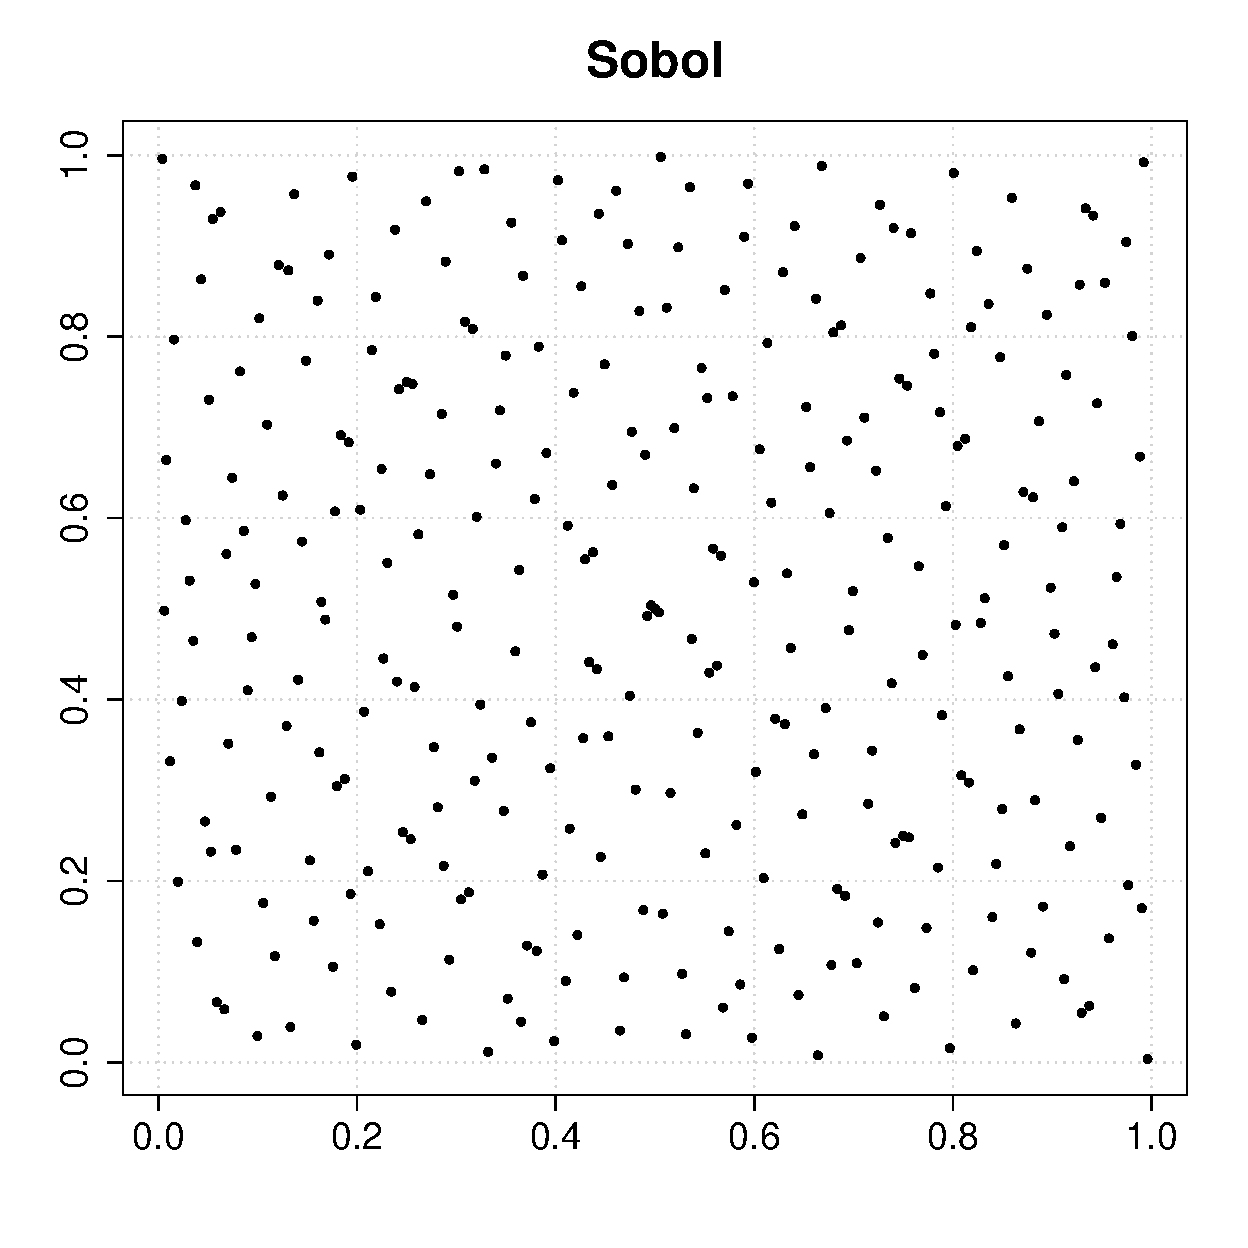
\includegraphics[width=0.95\textwidth]{sobol_cloud.pdf}
        \caption{Sobol sequence.}
        \label{Sobol}
      \end{center}
    \end{minipage}
    \hfill
    \begin{minipage}{0.5\textwidth}
      \begin{center}
        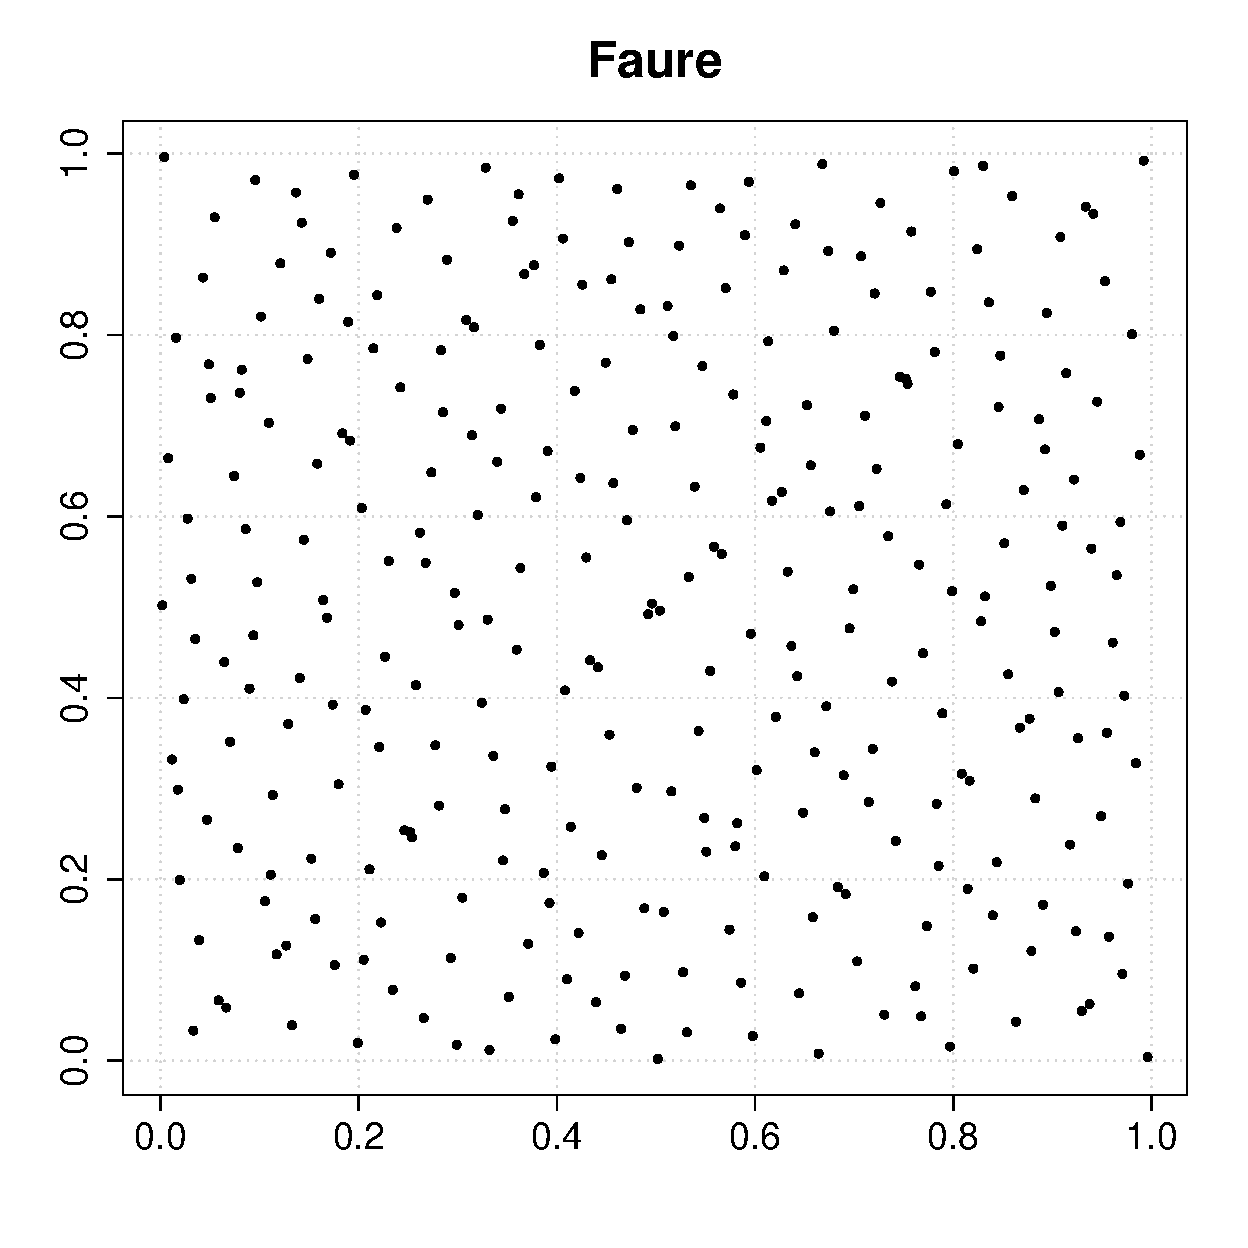
\includegraphics[width=0.95\textwidth]{faure_cloud.pdf}
        \caption{Faure sequence.}
        \label{Faure}
      \end{center}
    \end{minipage}
  \end{figure}

  \begin{figure}[H]
    \begin{minipage}{0.5\textwidth}
      \begin{center}
        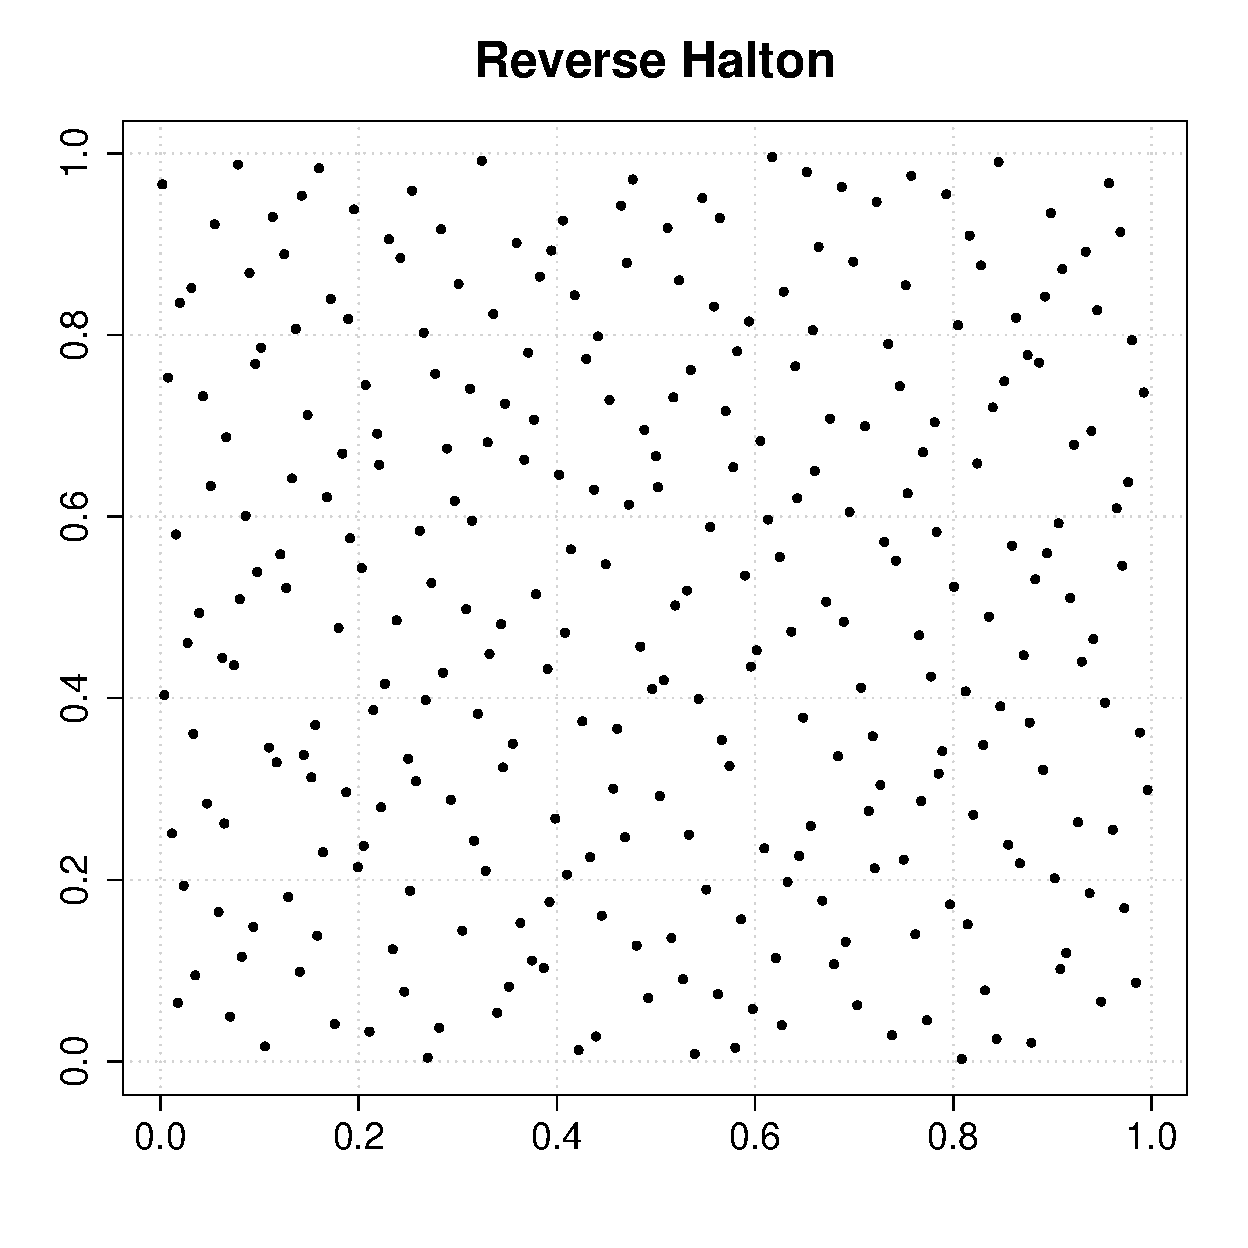
\includegraphics[width=0.95\textwidth]{reverseHalton_cloud.pdf}
        \caption{Reverse Halton sequence.}
        \label{ReverseHalton}
      \end{center}
    \end{minipage}
    \hfill
    \begin{minipage}{0.5\textwidth}
      \begin{center}
        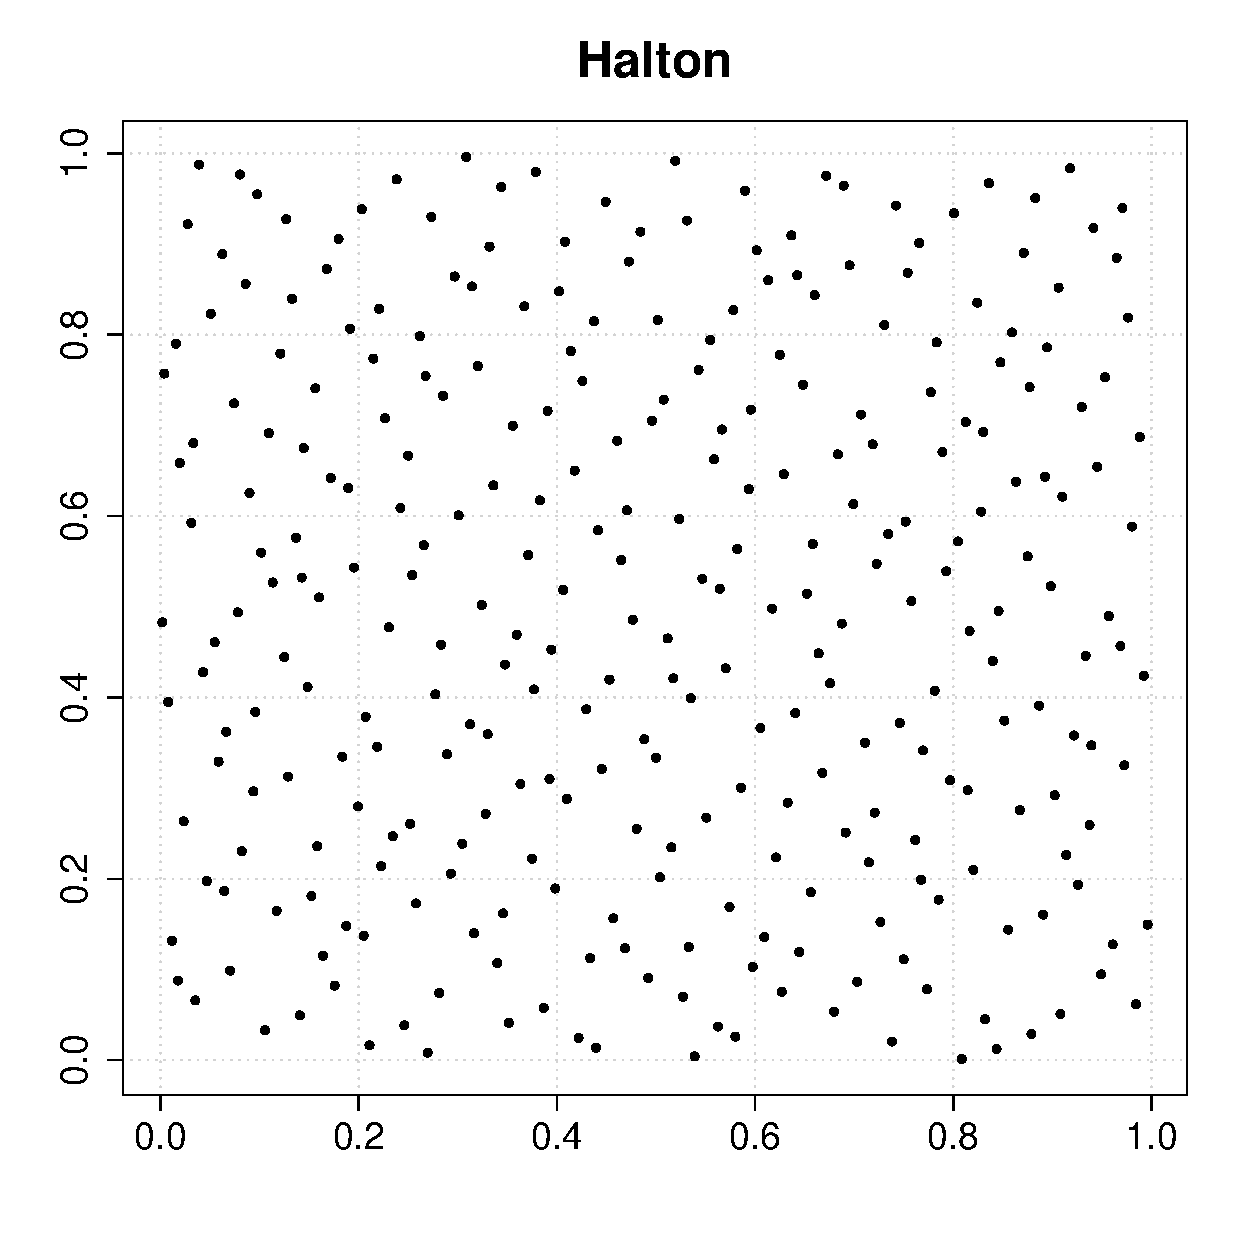
\includegraphics[width=0.95\textwidth]{halton_cloud.pdf}
        \caption{Halton sequence.}
        \label{Halton}
      \end{center}
    \end{minipage}
  \end{figure}

  \begin{figure}[H]
    \begin{minipage}{0.5\textwidth}
      \begin{center}
        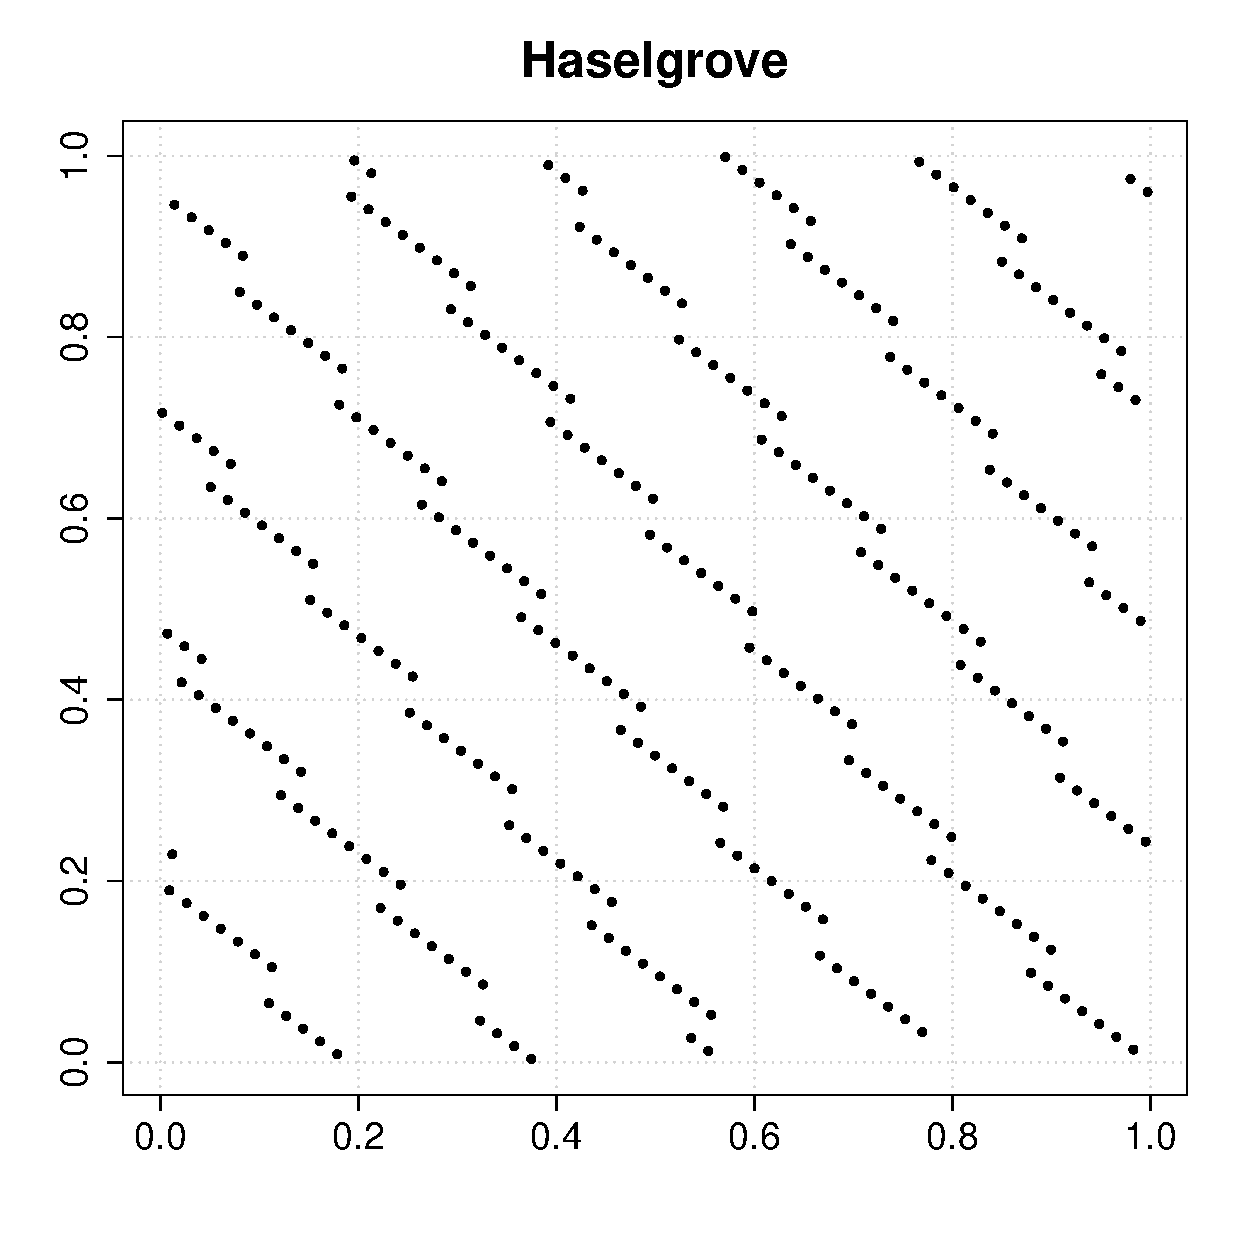
\includegraphics[width=0.95\textwidth]{haselgrove_cloud.pdf}
        \caption{Haselgrove sequence.}
        \label{Haselgrove}
      \end{center}
    \end{minipage}
    \hfill
    \begin{minipage}{0.5\textwidth}
      \begin{center}
        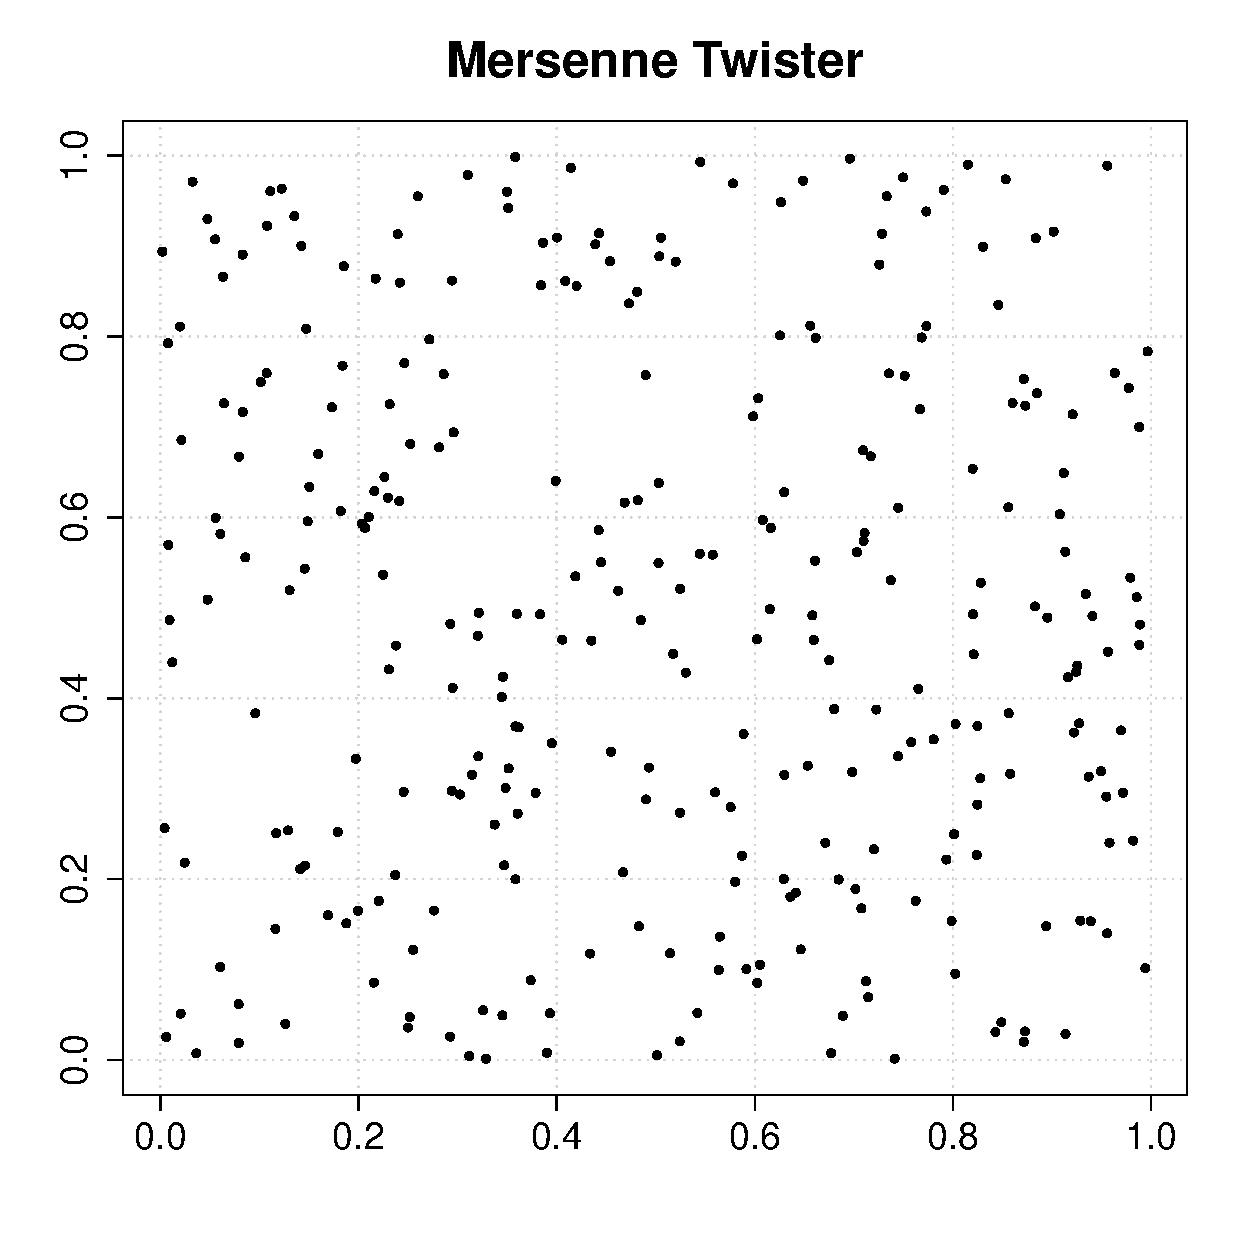
\includegraphics[width=0.95\textwidth]{mersenne_twister_cloud.pdf}
        \caption{Uniform random sequence.}
        \label{UniformRandom}
      \end{center}
    \end{minipage}
  \end{figure}

}
